\documentclass[11pt, a4paper]{article}
%\usepackage{proj1}
\usepackage{natbib}
\usepackage{fancyhdr}  
\usepackage{subcaption}
\usepackage{caption}
\usepackage{graphicx}
\usepackage{numprint}
\usepackage{multirow}
\linespread{1.25} 
\setlength{\parindent}{0cm}
\graphicspath{{Images/}}
\usepackage{hyperref}
\usepackage{amsmath}
\usepackage{amsfonts}
\usepackage{amssymb}
\usepackage{amsthm}
\usepackage{mathtools}
\usepackage{commath}
\usepackage{bbm}

%\usepackage[sc,osf]{mathpazo}
\usepackage{subcaption}
\usepackage[a4paper, top=1in, left=1.0in, right=1.0in, bottom=1in, includehead, includefoot]{geometry} %Usually have top as 1in

\usepackage{listings}
\usepackage{color} %red, green, blue, yellow, cyan, magenta, black, white
\definecolor{mygreen}{RGB}{28,172,0} % color values Red, Green, Blue
\definecolor{mylilas}{RGB}{170,55,241}


\hypersetup{colorlinks,linkcolor={black},citecolor={blue},urlcolor={black}}
\usepackage{color}
\urlstyle{same}


\theoremstyle{definition}
\newtheorem{definition}{Definition}[section]

%\newcommand{\Sta}{\rho}
\newcommand{\adja}{q_a}
\newcommand{\adjb}{q_b}
\newcommand{\adjaB}{q_{a,\partial \Omega}}
\newcommand{\adjbB}{q_{b,\partial \Omega}}
%\newcommand{\Con}{u}
\newcommand{\ra}{\rho_a}
\newcommand{\rb}{\rho_b}
\newcommand{\w}{\mathbf{w}}
\newcommand{\Stav}{\mathbf{v}}
\newcommand{\Adja}{\mathbf{p}}
\newcommand{\Adjb}{q}
\newcommand{\Adjc}{{p}_{\partial \Sigma}}
\newcommand{\Con}{\mathbf{f}}
\newcommand{\n}{\mathbf{n}}
\newcommand{\h}{\mathbf{h}}
\newcommand{\K}{\mathbf{K}}


\pagenumbering{gobble}
\begin{document}
	
	
\section{The Multiple Species Gradient Equation -- again}
We consider the derivative of the Lagrangian with respect to $\w$. However, we will need to consider the Frech\'et derivative of terms involving $F(\w)$ first. If $F$ is a function of $\w$ only and not of the position variable $r$, we can do the following. Otherwise, we will have to work with the definition of the Frech\'et derivative and derive the gradient equation like that.
We consider the first order term of the Taylor expansion, so that we have:
\begin{align*}
F(\w + \h) - F(\w) =  \bigg(\h \cdot \left(\frac{\partial}{\partial w_1}, \frac{\partial}{\partial w_2}\right)\bigg) F(\w) = h_1 \frac{\partial}{\partial w_1} F(\w)  + h_2\frac{\partial}{\partial w_2} F(\w) . 
\end{align*}
We denote this by $\h F'(\w)$, where $F'(\w)$ is scalar.
Then:
\begin{align*}
\mathcal{L}_{\w}(\ra,\rb, \w, \adja, \adjb) \h  &= \int_0^T \int_\Omega \bigg( \beta \w \cdot \h - D_a \nabla \cdot (\ra F_a'(\w)\h)  \adja - D_b \nabla \cdot (\rb F_b'(\w)\h) \adjb \bigg)dr dt \\
&+ \int_0^T \int_{\partial \Omega} \bigg( D_a \ra \adjaB F_a'(\w)\h  + D_b \rb \adjbB F_b'(\w)\h     \bigg) \cdot \n dr dt\\
&= \int_0^T \int_\Omega \bigg( \beta \w \cdot \h + D_a \nabla  \adja \cdot (\ra F_a'(\w) \h) 
+ D_b \nabla \adjb \cdot (\rb F_b'(\w) \h) \bigg)dr dt \\
&- \int_0^T \int_{\partial \Omega} \bigg( D_a \ra \adjaB F_a'(\w)\h  + D_b \rb \adjbB F_b'(\w)\h     \bigg) \cdot \n dr dt\\
&+\int_0^T \int_{\partial \Omega} \bigg( D_a \ra \adja F_a'(\w)\h  + D_b \rb \adjb F_b'(\w) \h     \bigg) \cdot \n dr dt\\
&= \int_0^T \int_\Omega \bigg( \beta \cdot \w \h + D_a \nabla  \adja \cdot (\ra F_a'(\w) \h) 
+ D_b \nabla \adjb \cdot (\rb F_b'(\w)\h) \bigg)dr dt,
\end{align*}
since $\adja = \adjaB$ and $\adjb = \adjbB$ from the adjoint derivation.\\
Since this holds for all permissible $\h$, we get:
\begin{align*}
\w  = - \frac{1}{\beta} \bigg( D_a  \ra F_a'(\w)\nabla  \adja 
+ D_b  \rb F_b'(\w) \nabla \adjb\bigg).
\end{align*} 
As an example, take $F_a(\w) = c_a \w$ and $F_b(\w) = c_b \w$. We get:
\begin{align*}
\w  = \frac{1}{\beta}\bigg( D_a c_a  \ra  \nabla \adja + D_b c_b \rb \nabla \adjb \bigg).
\end{align*}	
	
\section{Sedimentation}	
	
	\subsection{Free Energy}
	We need to calculate the equation of motion from the given free energy. Here we consider the part that's not done before (i.e. excluding the $V_{ext}$ and $V_2$ terms).
	We have the following free energy functional:
	\begin{align*}
	F[\rho] &= \frac{1}{\beta} \int \rho (\ln \Lambda^2 \rho) - 2 \rho - \rho \ln(1 - \eta) + \frac{\rho}{1 - \eta} dr\\
	\eta &= a \rho = \frac{\pi \sigma^2}{4} \rho
	\end{align*}
	Taking the functional derivative of $F$ gives:
	\begin{align*}
	\frac{\delta F[\rho]}{\delta \rho} &= \frac{1}{\beta} \bigg(1 + \ln \rho + \Lambda^2 -2 - \ln(1-\eta) + a \frac{\rho}{1 - \eta} + \frac{1}{1 - \eta} + a \frac{\rho}{(1 - \eta)^2}  \bigg)\\
	&= \frac{1}{\beta} \bigg(1 + \ln \rho + \Lambda^2 -2 - \ln(1-\eta) + \frac{1}{(\eta - 1)^2} - \frac{1}{\eta - 1}  - 1\bigg)\\
	&= \frac{1}{\beta} \bigg( \ln \rho + \Lambda^2 - 2 - \ln(1-\eta) - \frac{\eta - 2}{(\eta - 1)^2}  \bigg),
	\end{align*}
	using partial fractions.
	\begin{align*}
	\nabla \frac{\delta F[\rho]}{\delta \rho} &= \frac{1}{\beta} \bigg( \nabla\ln \rho + \nabla(\Lambda^2 - 2) - \nabla\ln(1-\eta) - \nabla\frac{\eta - 2}{(\eta - 1)^2}  \bigg)\\
	& = \frac{1}{\beta} \bigg( \frac{\nabla \rho}{\rho} - \frac{\nabla( 1- \eta)}{1 - \eta} - \nabla\frac{\eta - 2}{(\eta - 1)^2}  \bigg)\\
	& = \frac{1}{\beta} \bigg( \frac{\nabla \rho}{\rho} + \frac{\nabla \eta}{1 - \eta} - \nabla\frac{\eta - 2}{(\eta - 1)^2}  \bigg)
	\end{align*}
	Then multiplying by $\rho$ gives:
	\begin{align*}
	\rho \nabla \frac{\delta F[\rho]}{\delta \rho} &= \frac{1}{\beta} \bigg( \nabla \rho +   \frac{\rho \nabla \eta}{1 - \eta} - \rho \nabla\frac{\eta - 2}{(\eta - 1)^2}  \bigg)\\
	&= \frac{1}{\beta} \bigg( \nabla \rho +   \frac{\eta\nabla \rho}{1 - \eta} - \rho \nabla\frac{\eta - 2}{(\eta - 1)^2}  \bigg)\\
	&= \frac{1}{\beta} \bigg( \nabla \rho + \frac{\nabla \rho}{1 - \eta} - \nabla \rho - \rho \nabla\frac{\eta - 2}{(\eta - 1)^2}  \bigg)\\
	&= \frac{1}{\beta} \bigg(  \frac{\nabla \rho}{1 - \eta}  - \rho \nabla\frac{\eta - 2}{(\eta - 1)^2}  \bigg)
	\end{align*}
	Finally we take the divergence:
	\begin{align*}
	\nabla \cdot \bigg(\rho \nabla \frac{\delta F[\rho]}{\delta \rho}\bigg) &= \frac{1}{\beta} \bigg( \nabla  \cdot \left(  \frac{\nabla \rho}{1 - \eta} \right) - \nabla  \cdot \left(\rho \nabla\frac{\eta - 2}{(\eta - 1)^2} \right) \bigg)\\
	&= \frac{1}{\beta} \bigg( \frac{\nabla^2 \rho}{1 - \eta} +  \nabla \rho \cdot \nabla \frac{1}{1 - \eta} - \nabla \rho \cdot \nabla \frac{\eta - 2}{(\eta - 1)^2} - \rho \nabla^2\frac{\eta - 2}{(\eta - 1)^2} \bigg)\\
	&= \frac{1}{\beta} \bigg( \frac{\nabla^2 \rho}{1 - \eta} +  \nabla \rho \cdot \nabla \frac{(3- 2 \eta)}{(1 - \eta)^2}  - \rho \nabla^2\frac{\eta - 2}{(\eta - 1)^2} \bigg)
	\end{align*}
	
\subsection{Redoing Archer's results}
	First of all, the paper contains a different potential to our standard one:
	\begin{align*}
	V_2 = exp(-r/\sigma),
	\end{align*}
	where $\sigma$ is the particle diameter of the hard sphere particle.
	Then we have the following quantities to choose:
	$\sigma$, $\Omega$, which depends on $\sigma$. In the paper we have $L_y = 43.5 \sigma$, and I guesstimate that $L_x = 60$ from the graphs. 
	We then have the strength of the external potential given by $\beta a = 0.1$ and the strength of the interaction term $\epsilon$ is given by $\beta \epsilon = 3.5$, where $\beta = \frac{1}{k_BT}$. 
	Furthermore, we have the average density of the system $\bar \rho \sigma^2$, calculated using $(1/L_y)\int_0^L \rho \sigma^2 dy$.
	The initial condition for $\rho$ is found by considering $\bar \rho$ and adding a uniform random number to each location in the range $\pm \bar \rho/ 20$.
	\subsubsection{Example Figure 8}
	For simplicity I set $\beta = 1$ everywhere. I then set $\sigma = 1$, which gives for the example in Figure 8 that $\bar \rho = 0.072$. However, I am scaling the domain, and choose $L_y = 21$, $L_x = 30$ but $\bar \rho = 0.072$. We further have $\epsilon = 3.5$, $a = 0.1$
	I choose $n = 30$, $N = 40$ and we run this up to time $30$. If we were to instead increase the strength of $V_{ext}$, we would see the sediment flatten out more at the bottom. The result, which takes $12$ seconds to run, can be seen in Figure \ref{F1}. 
	\begin{figure}[h]
		\centering
		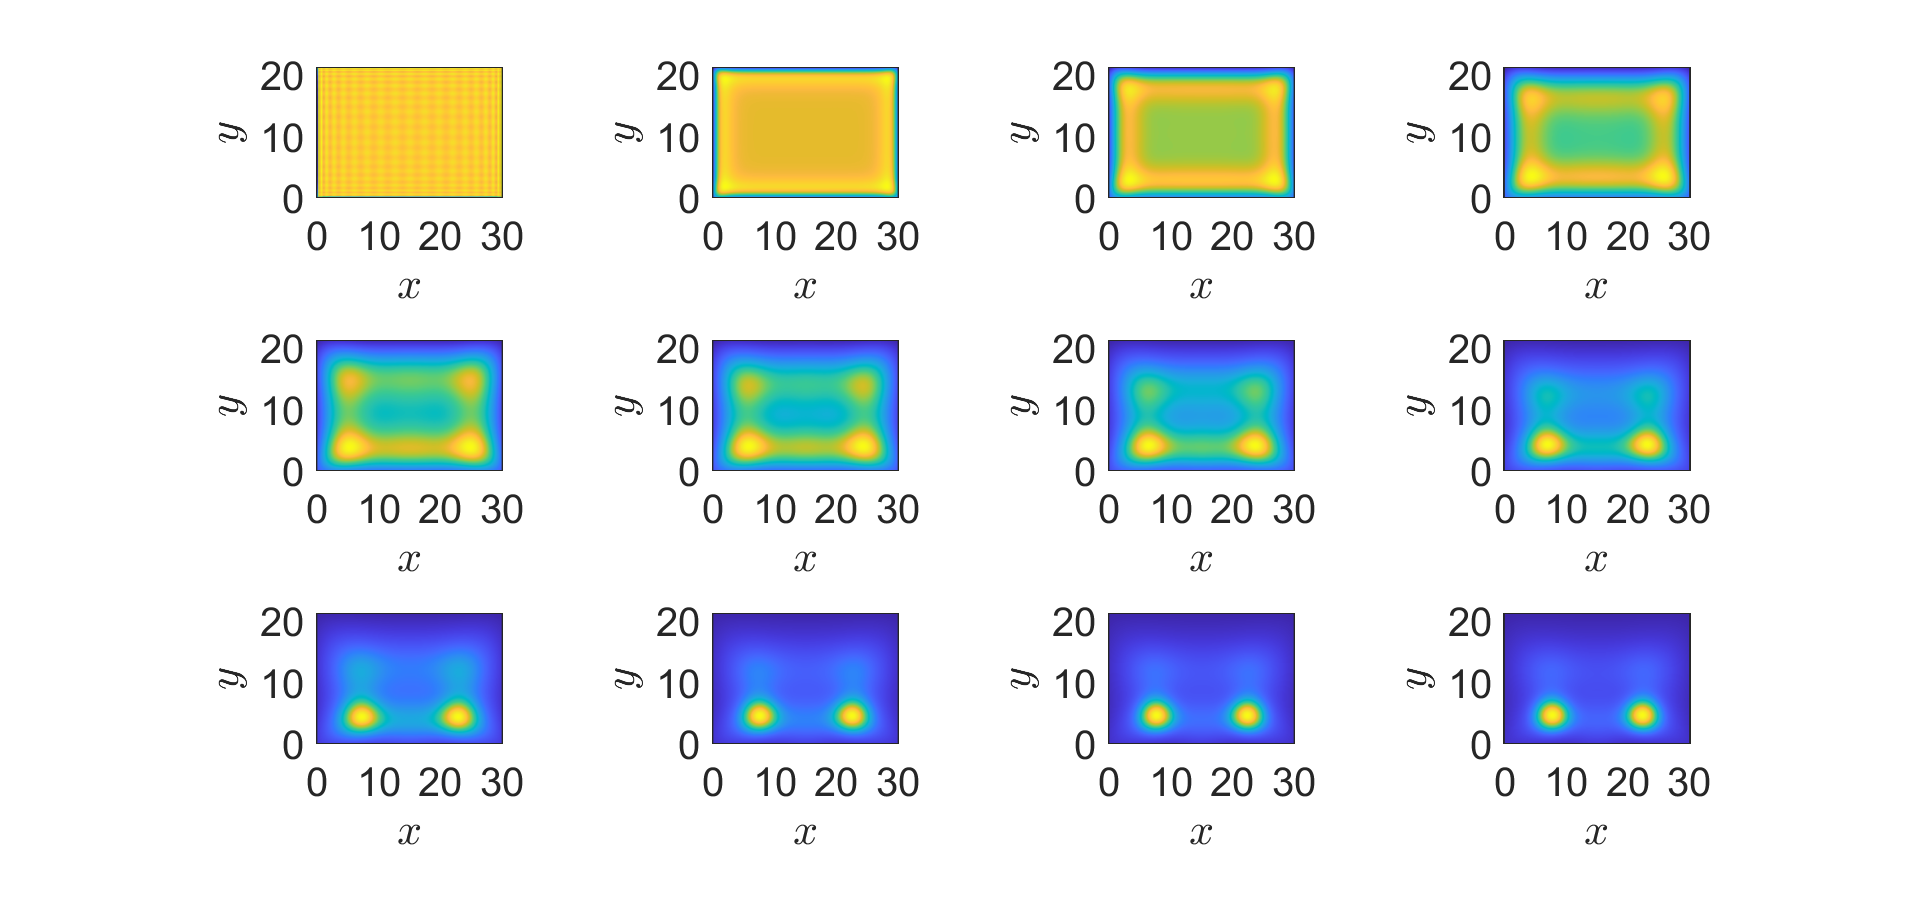
\includegraphics[scale=0.35]{Ex8F1.png}
		\caption{Figure 8 Example, $\bar \rho = 0.072$, $\sigma = 1$, $12$ different times} 
		\label{F1}
	\end{figure} 
 
	
	
	Next, we decrease $\sigma$ to get closer to the scaling from the paper. We set $\sigma = 0.8$. Inspecting the result, it is clear that it needs more points, so we run it with $N = 50$ instead. This increases running time from $30$ seconds to $2$ min. In Figure \ref{F2} we can see that a third cluster is building. 
	\begin{figure}[h]
		\centering
		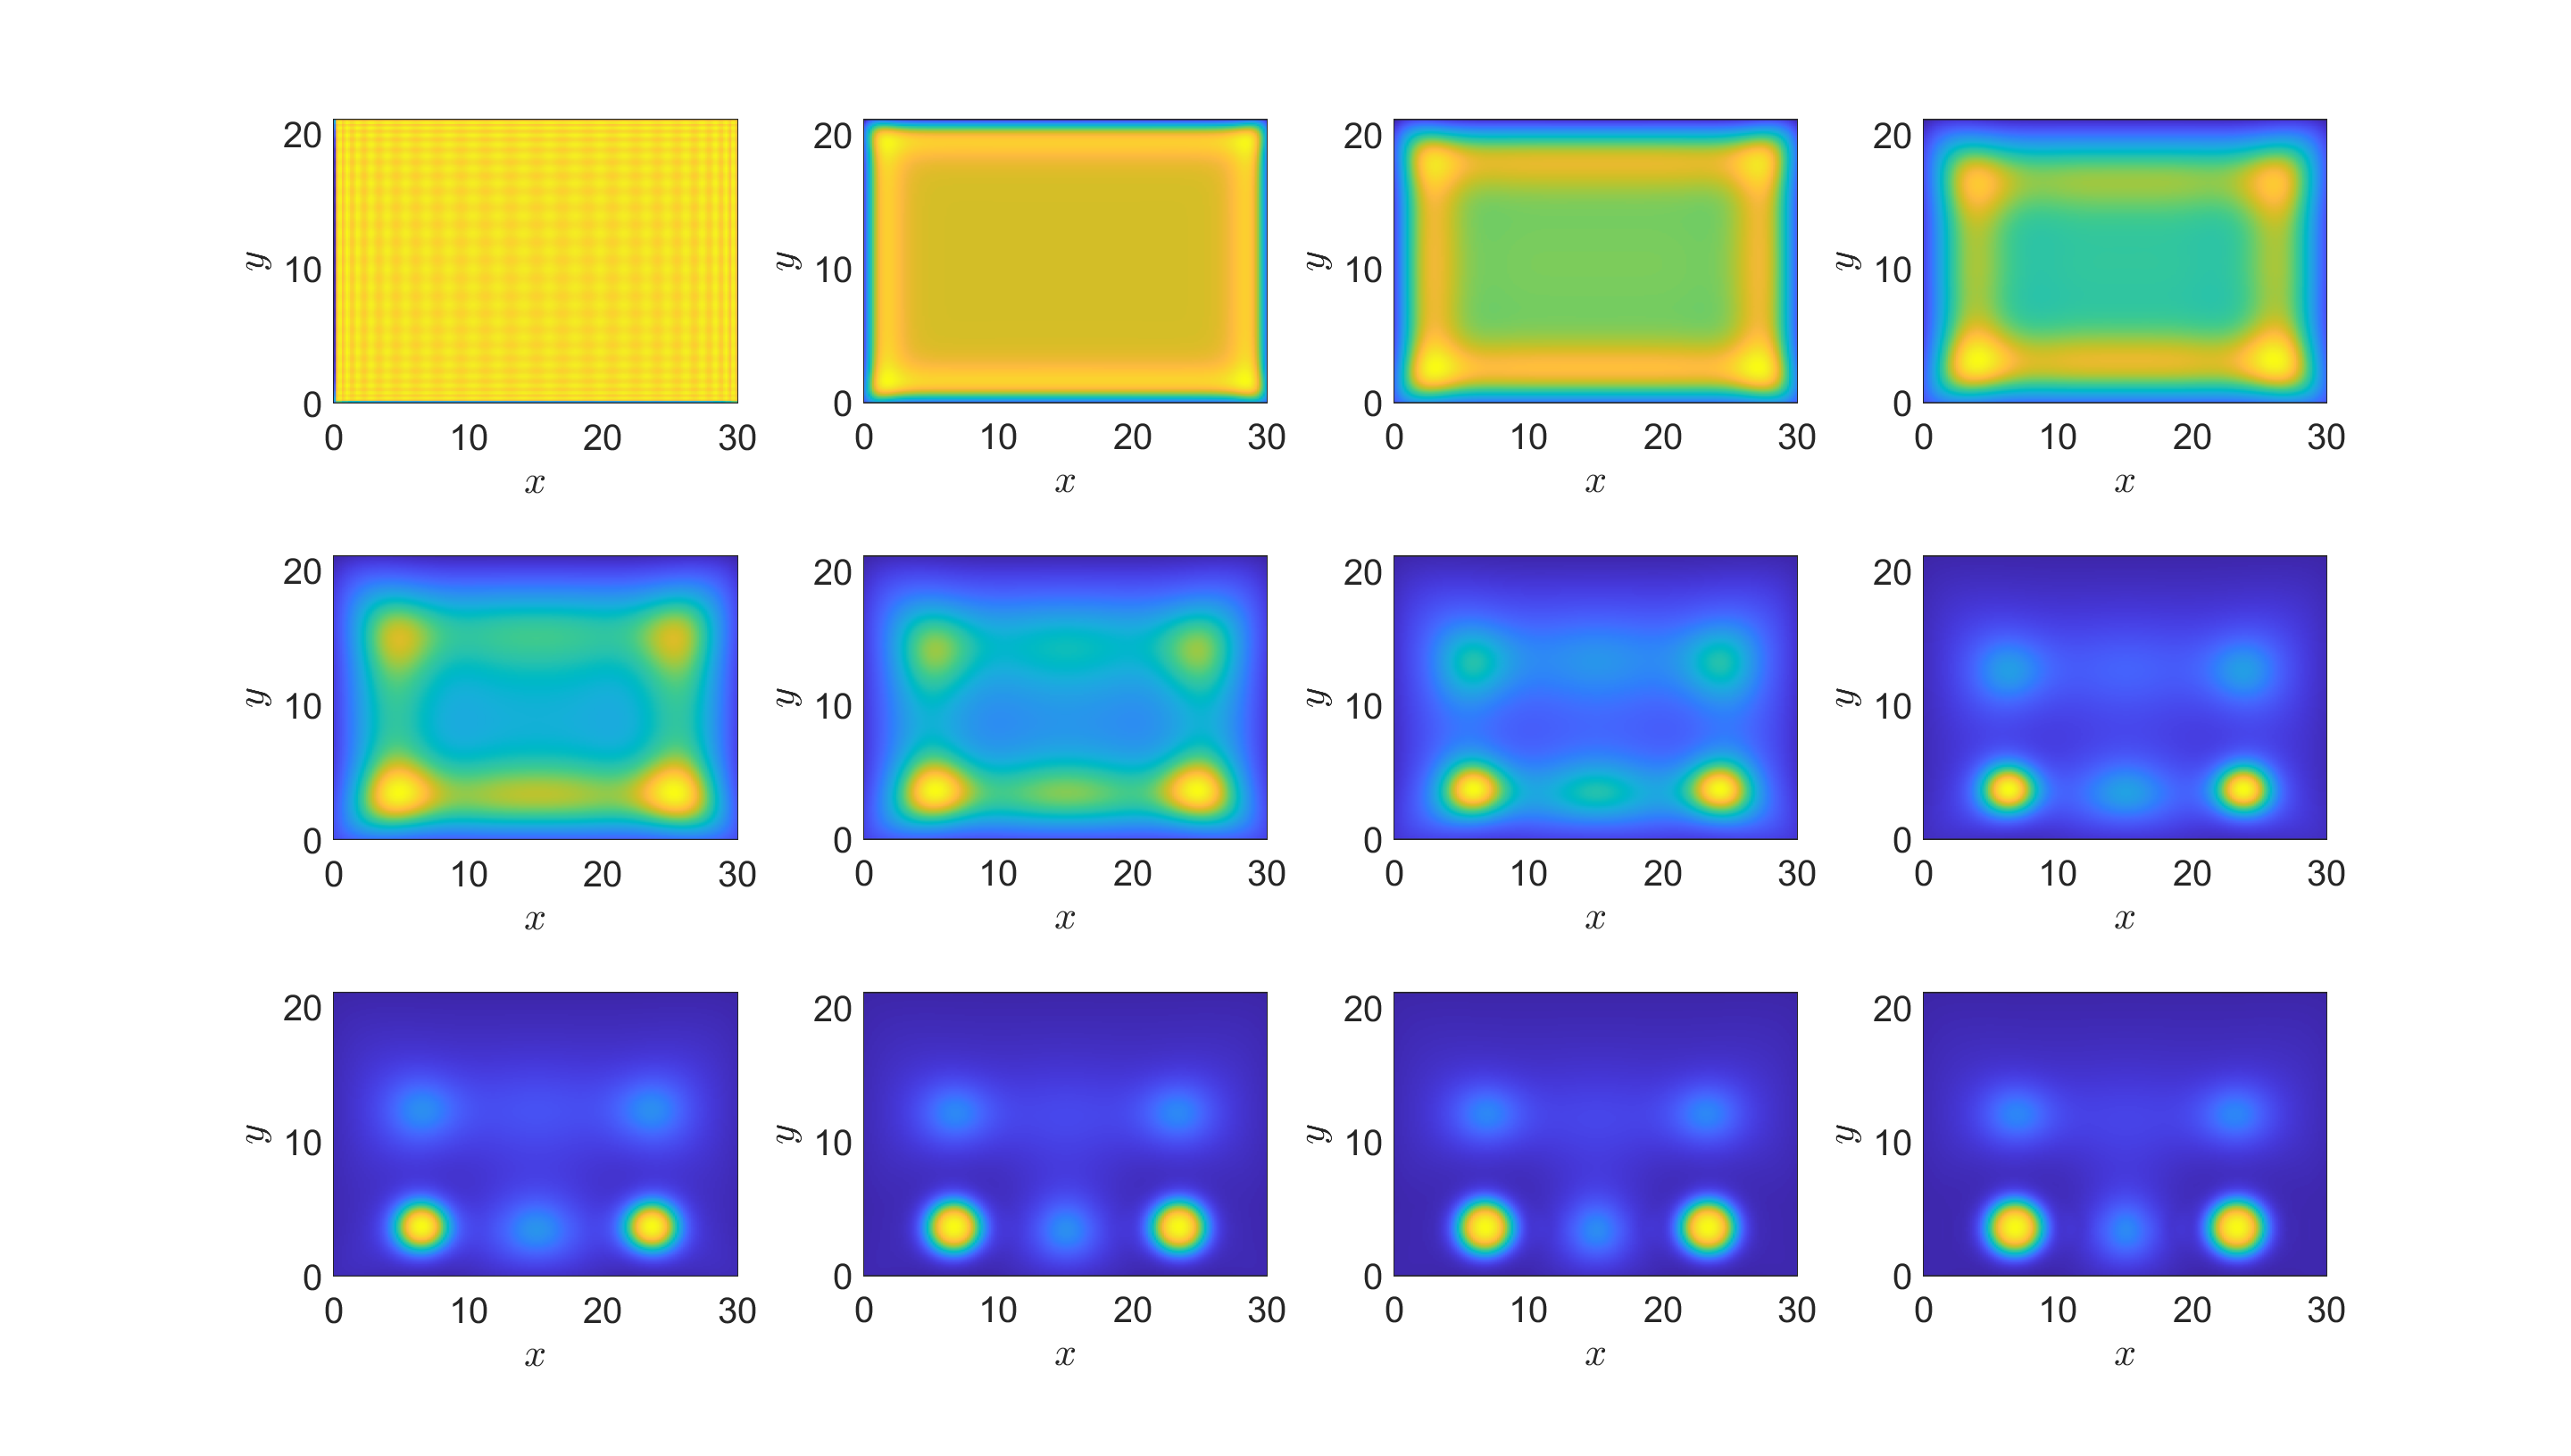
\includegraphics[scale=0.25]{Ex8F2.png}
		\caption{Figure 8 Example, $\bar \rho = 0.072$, $\sigma = 0.8$, $12$ different times} 
		\label{F2}
	\end{figure} 
	If we decrease $\sigma$ to $0.6$ we again need more points. We try $N = 60$, which takes $14$ min and is still not enough. This can be seen in Figure \ref{F3}. We can see that more clusters are building but it's numerically not good and would need to be run again. This configuration is closest to the actual model setup because we have half of the domain that Archer has, so we need to half $\sigma$.
	\begin{figure}[h]
		\centering
		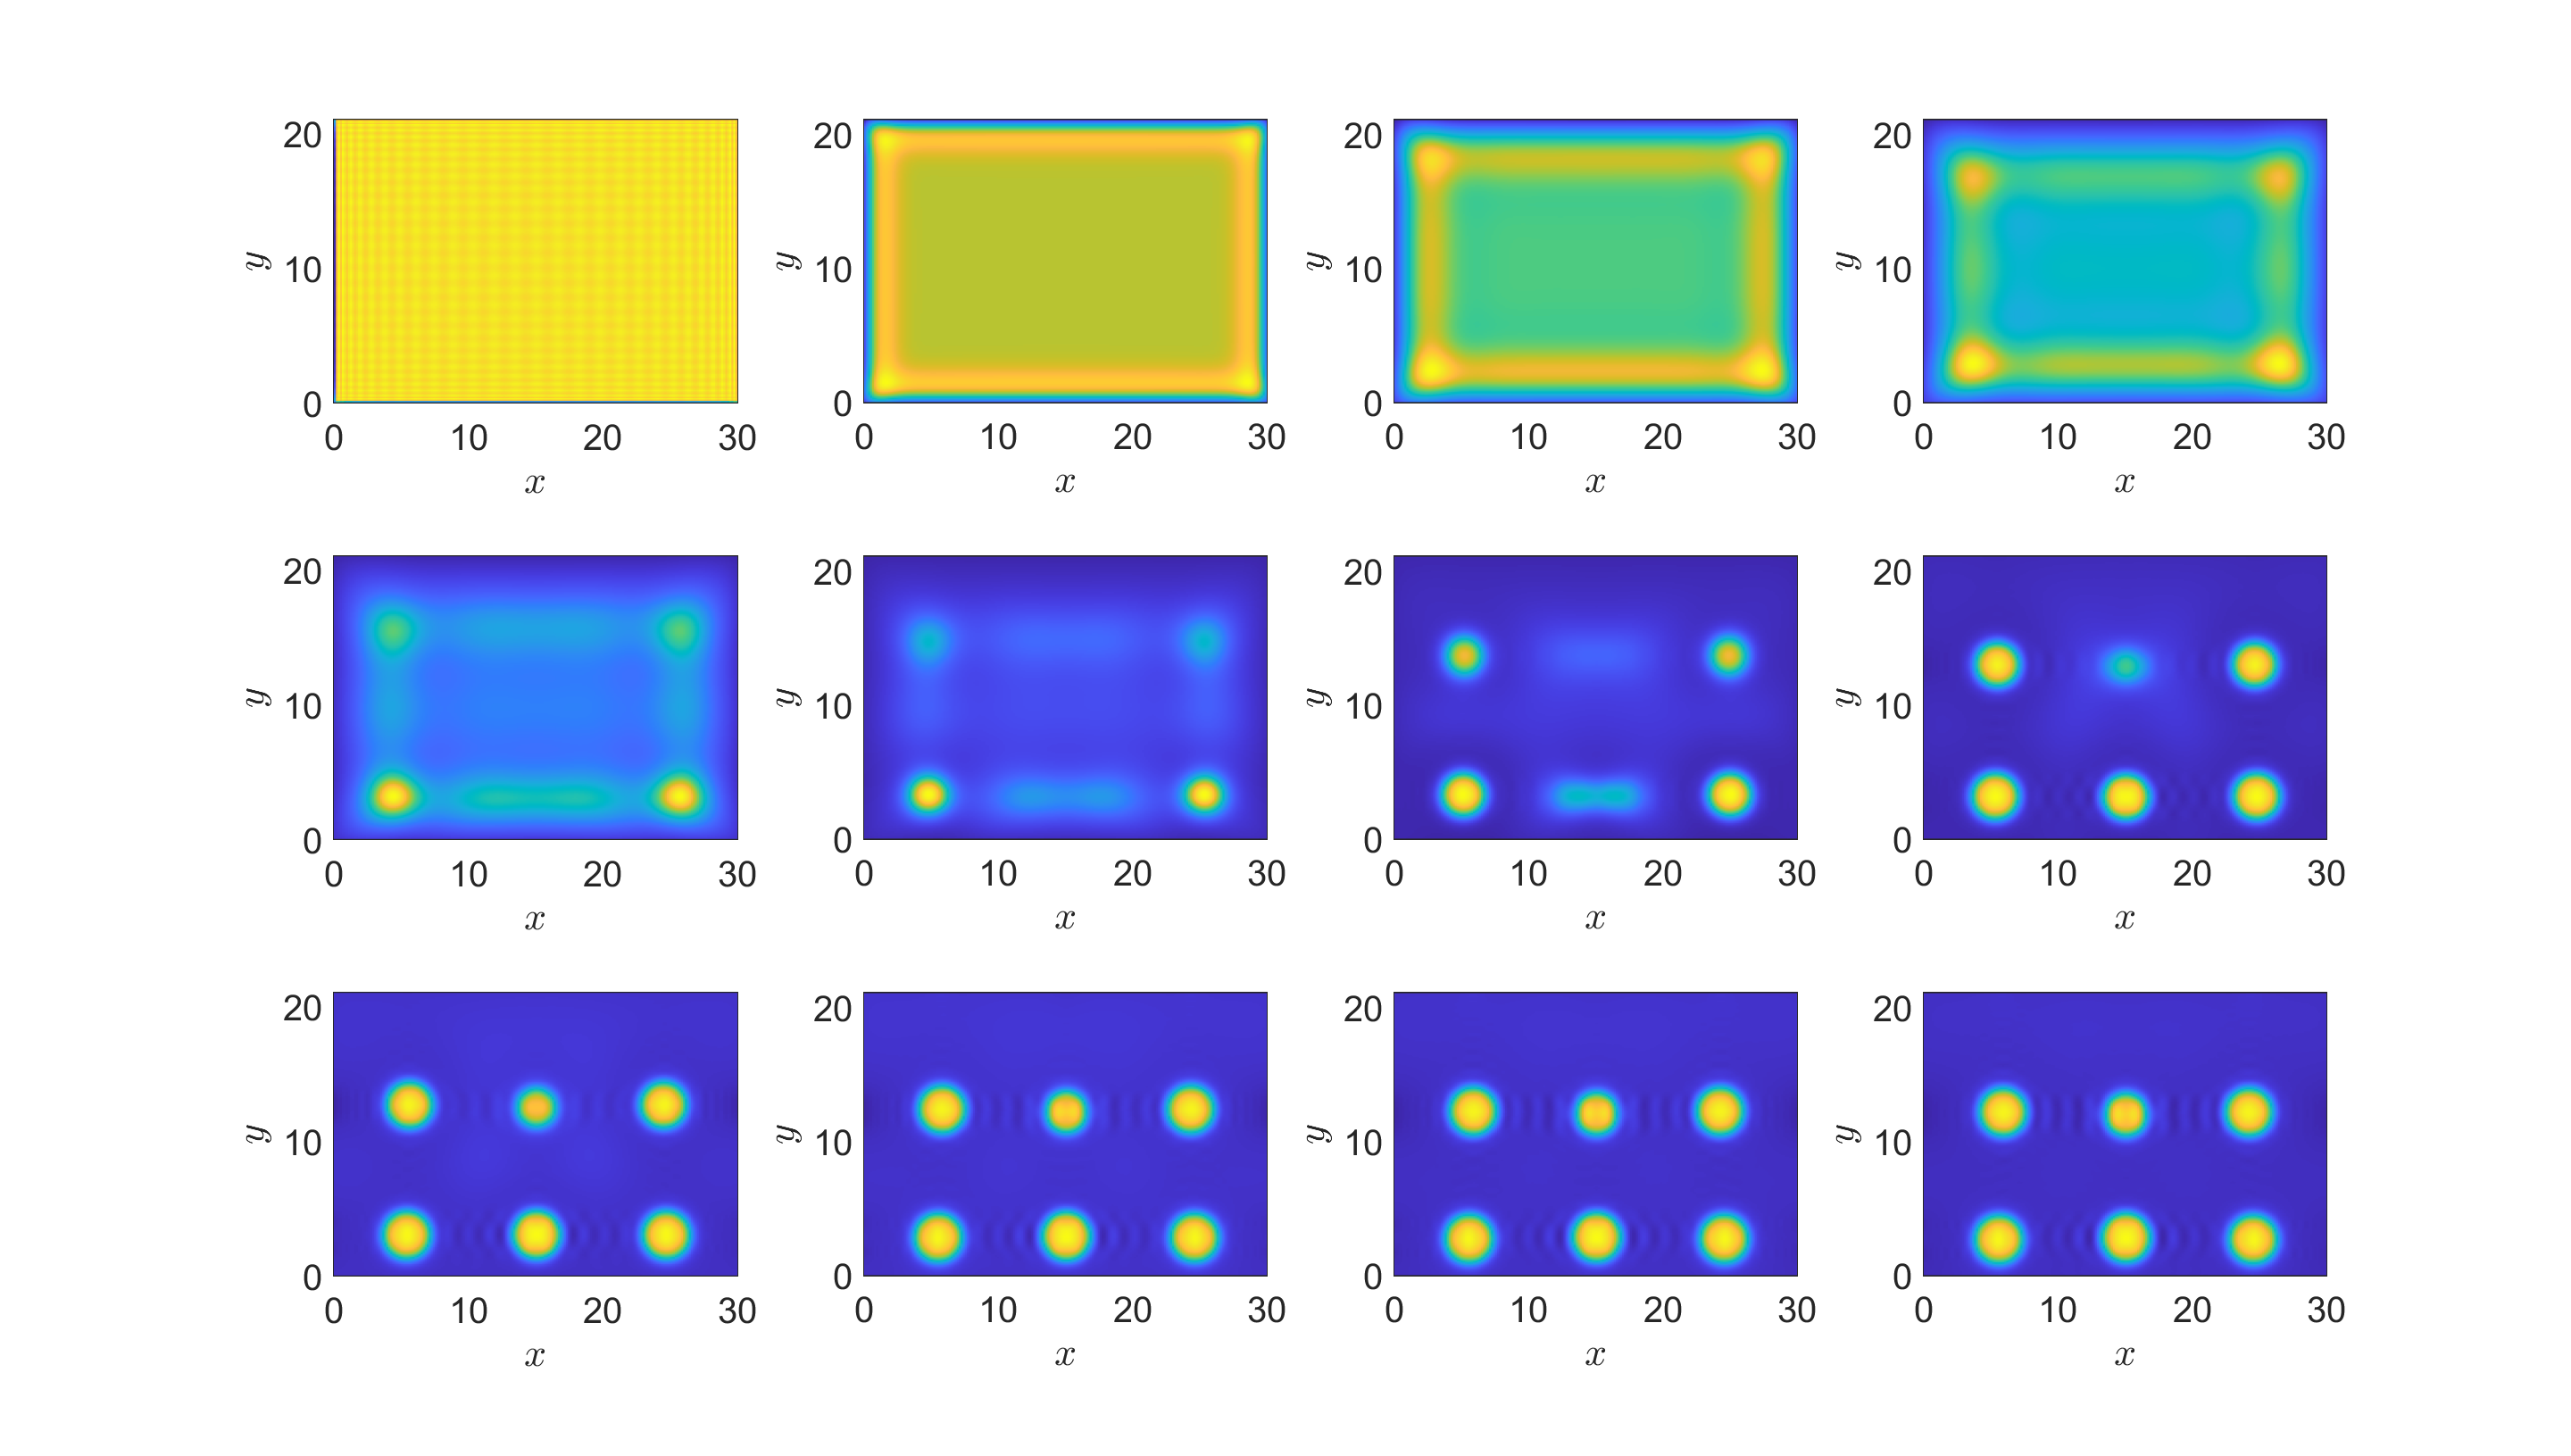
\includegraphics[scale=0.25]{Ex8F3.png}
		\caption{Figure 8 Example, $\bar \rho = 0.072$, $\sigma = 0.5$, $12$ different times} 
		\label{F3}
	\end{figure} 

	
	\begin{figure}[h]
		\centering
		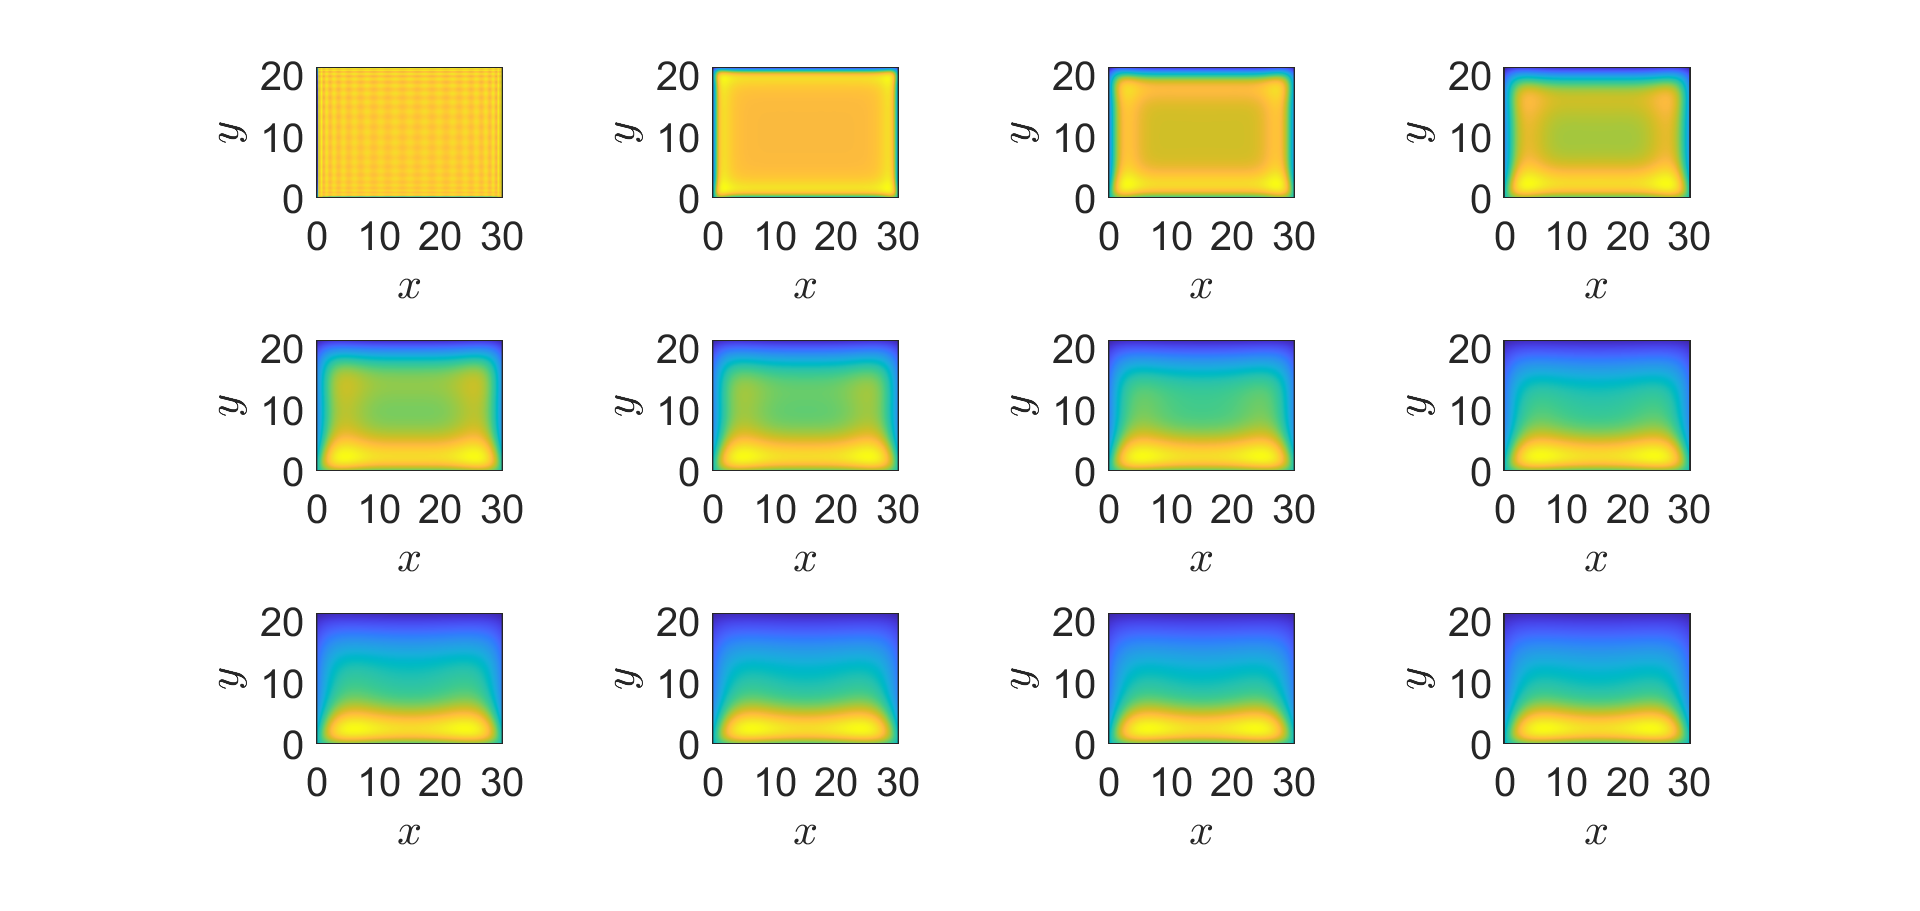
\includegraphics[scale=0.35]{Ex8F1b.png}
		\caption{Figure 8 Example, $\bar \rho = 0.036$, $\sigma = 1$, $12$ different times} 
		\label{F1b}
	\end{figure}
	If I instead decrease $\bar \rho$  to $0.036$, the sediment is more spread out at the bottom, which to me is counter-intuitive because scaling wise this should be the same as $\sigma = 0.7$, see Figure \ref{F1b}. Maybe I don't quite understand how this works.
	
	Just out of interest I change the initial condition to be non-symmetric: $\bar \rho = 0.072 *(1 + cos(\pi / 30 y_1)cos(\pi / 30 y_2))$. This has the effect that the final distribution is asymmetric as well, see Figure \ref{Fx}. This is done with $N = 40$ which is again not quite enough for numerical stability, but it takes $1$ min $20$ seconds to solve.
	\begin{figure}[h]
		\centering
		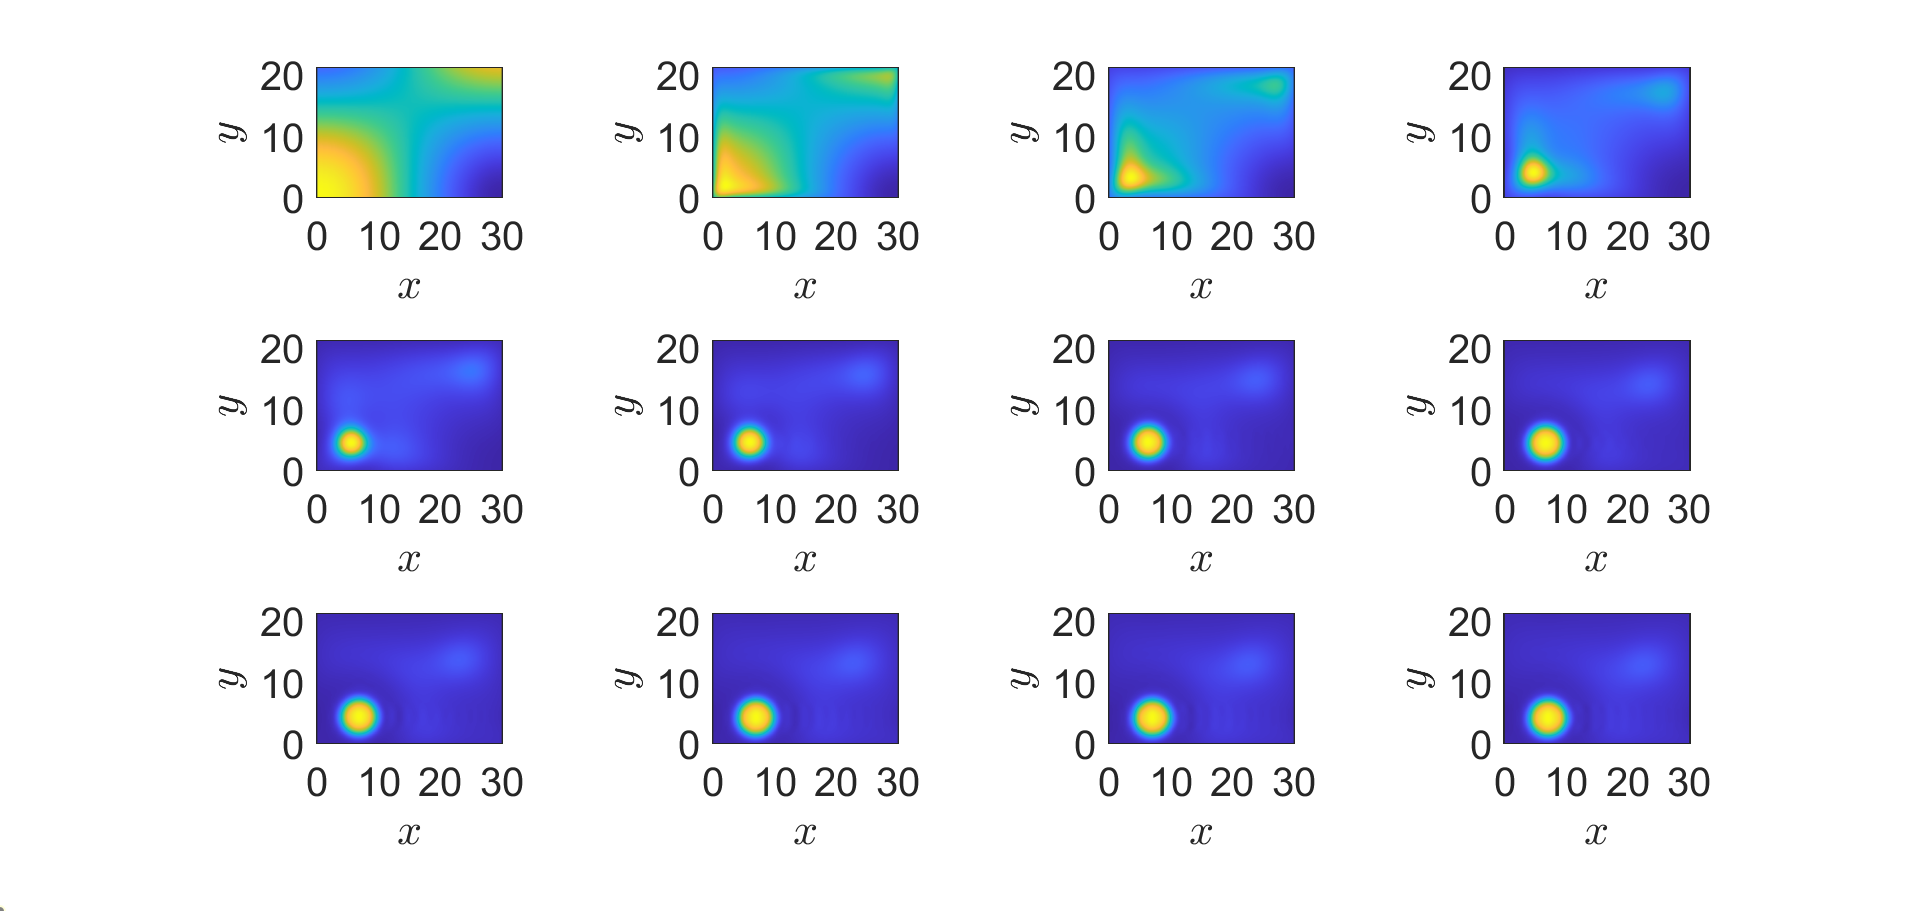
\includegraphics[scale=0.4]{Ex8NonSym.png}
		\caption{Figure 8 Example, $\bar \rho = 0.072$, $\sigma = 1$, $12$ different times, asymmetric initial condition} 
		\label{Fx}
	\end{figure}
	\subsubsection{Example Figure 10}
	In this example everything stays the same except that more density is in the system, $\bar \rho \sigma^2 = 0.2$. We start with $\sigma = 1$ and $\bar \rho = 0.2$, which needs more points. We try $N = 50$. This is still not quite enough but better and takes $8$ minutes to solve, see Figure \ref{F4}. We can see the sort of behaviour that is visible in the paper, that the different clusters merge. I think if we let time run longer it'd merge into one.
	\begin{figure}[h]
		\centering
		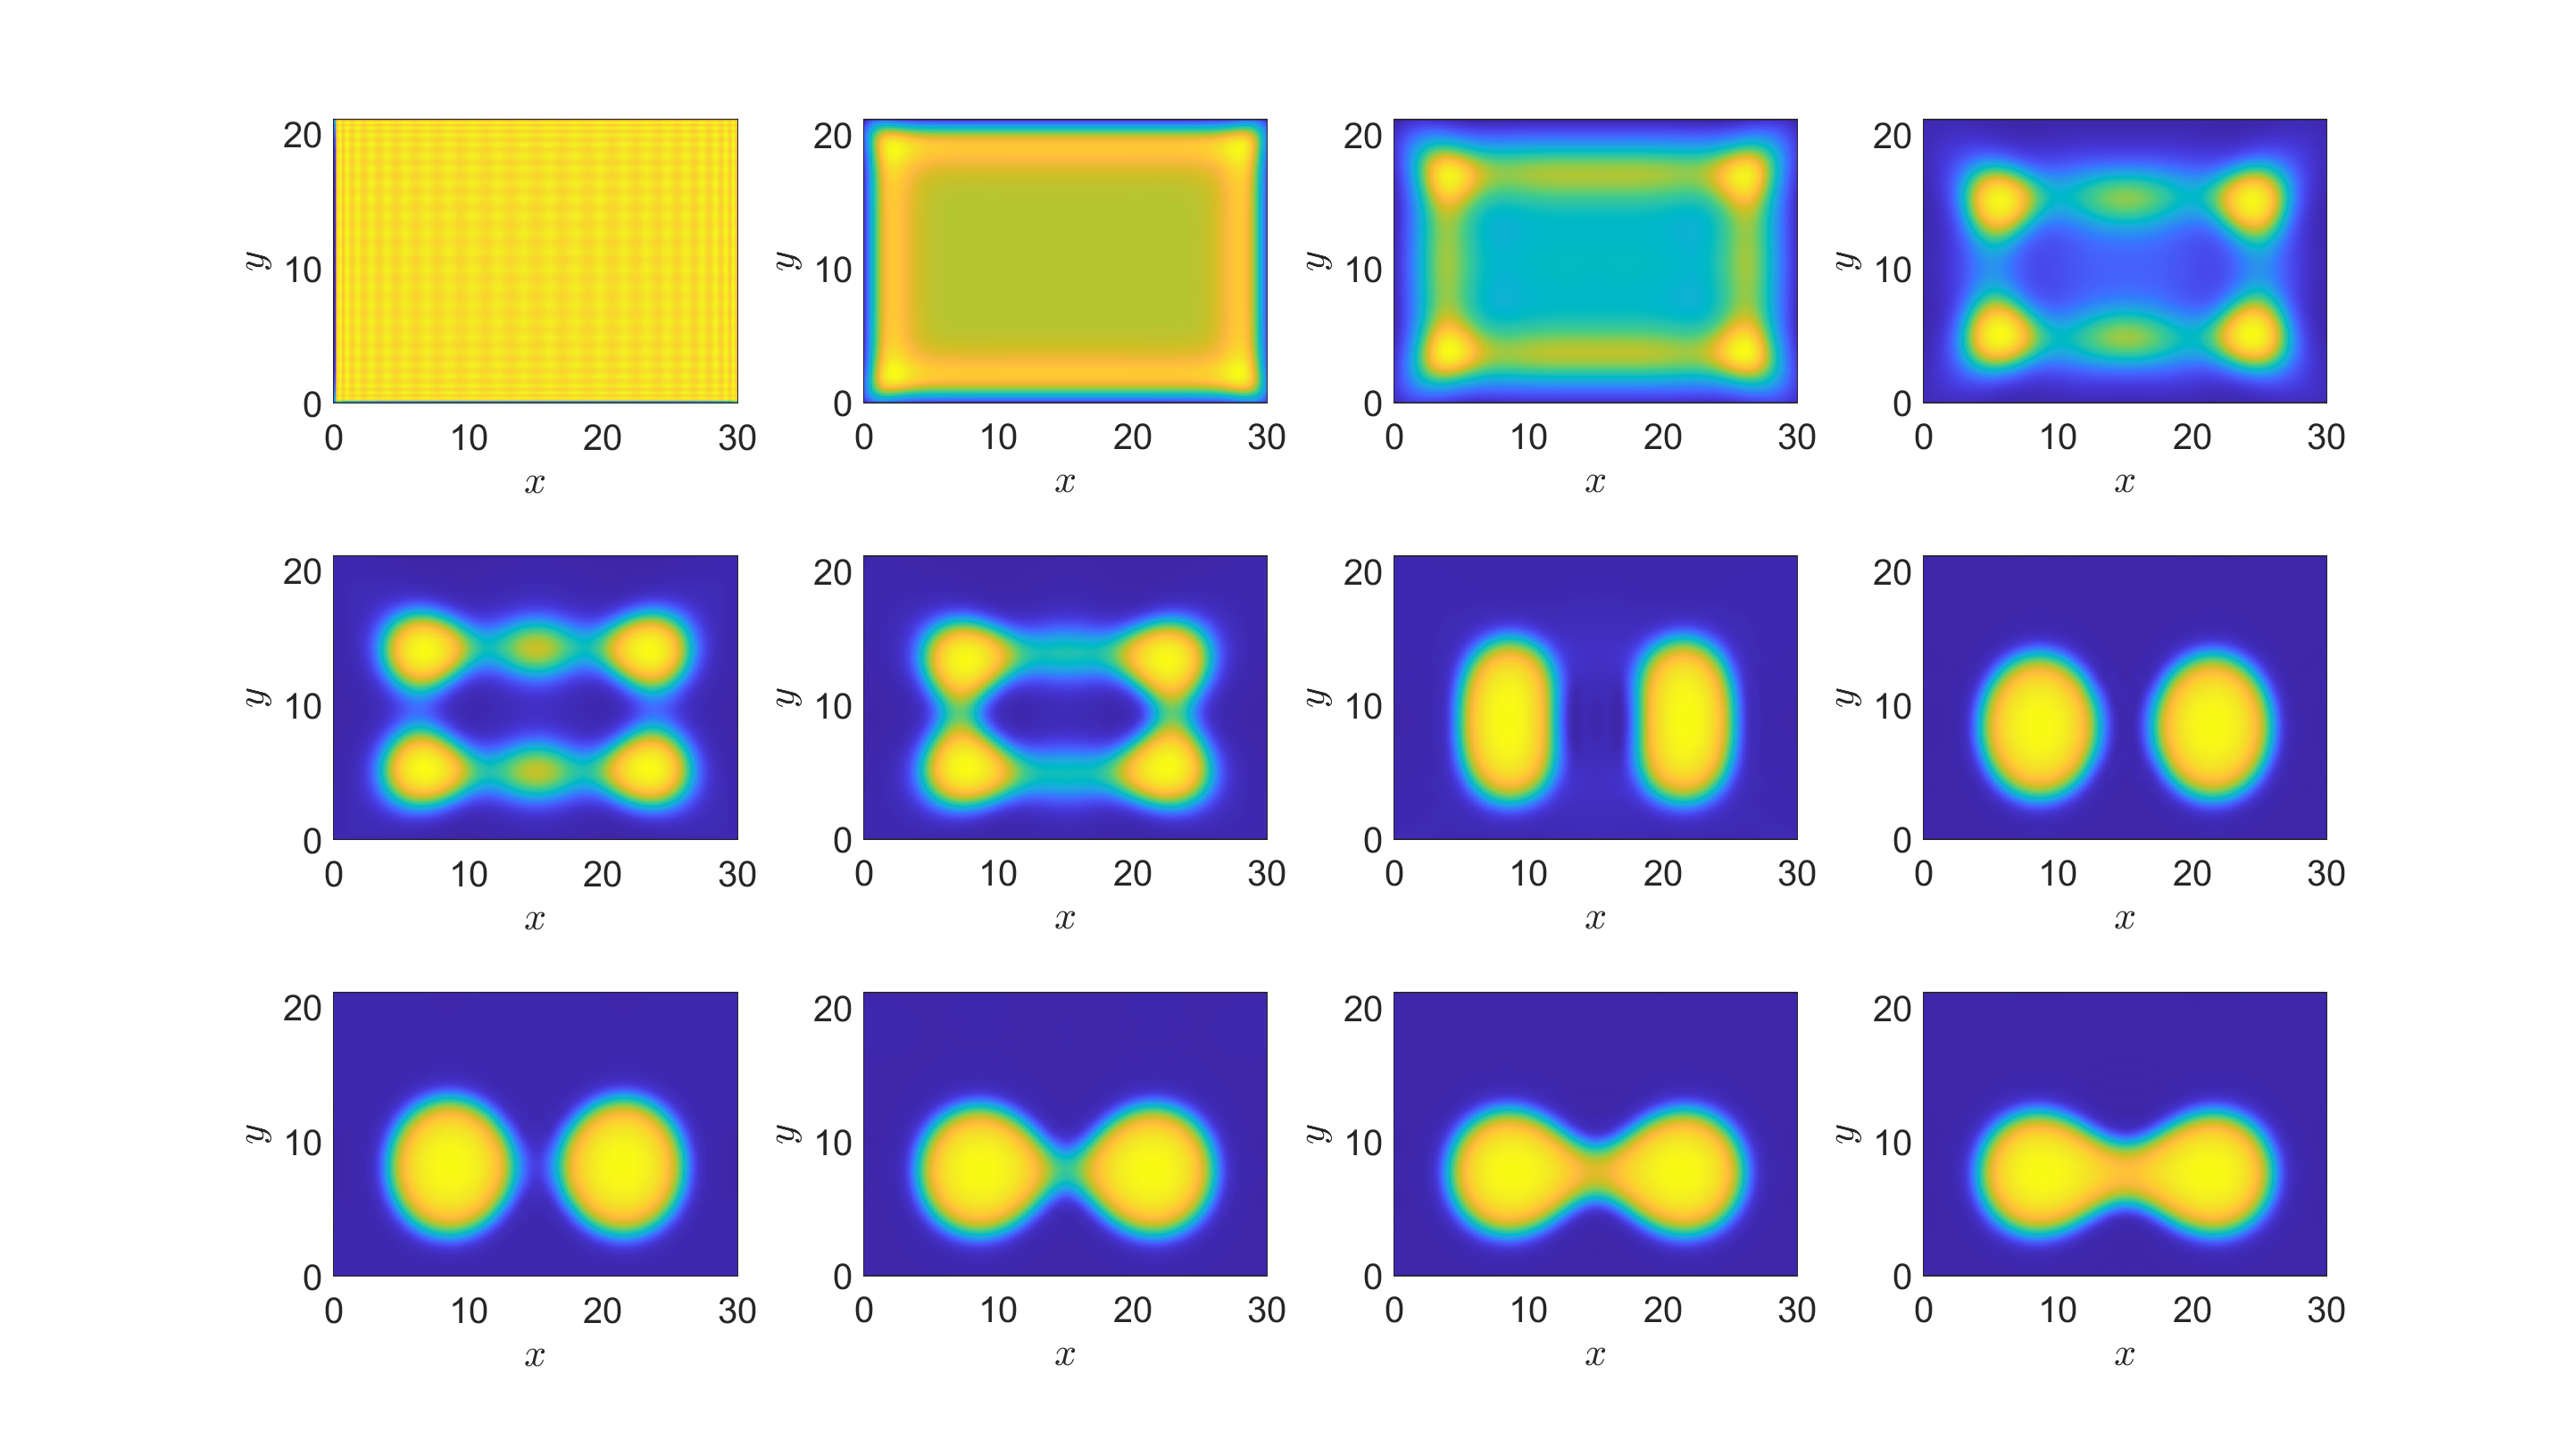
\includegraphics[scale=0.25]{Ex10F1.png}
		\caption{Figure 10 Example, $\bar \rho = 0.2$, $\sigma = 1$, $12$ different times} 
		\label{F4}
	\end{figure} 
	Again, since we have half the domain we set $\sigma = 0.6$. We use $60$ points but that's not enough again as can be seen in Figure \ref{F4b}.
	\begin{figure}[h]
		\centering
		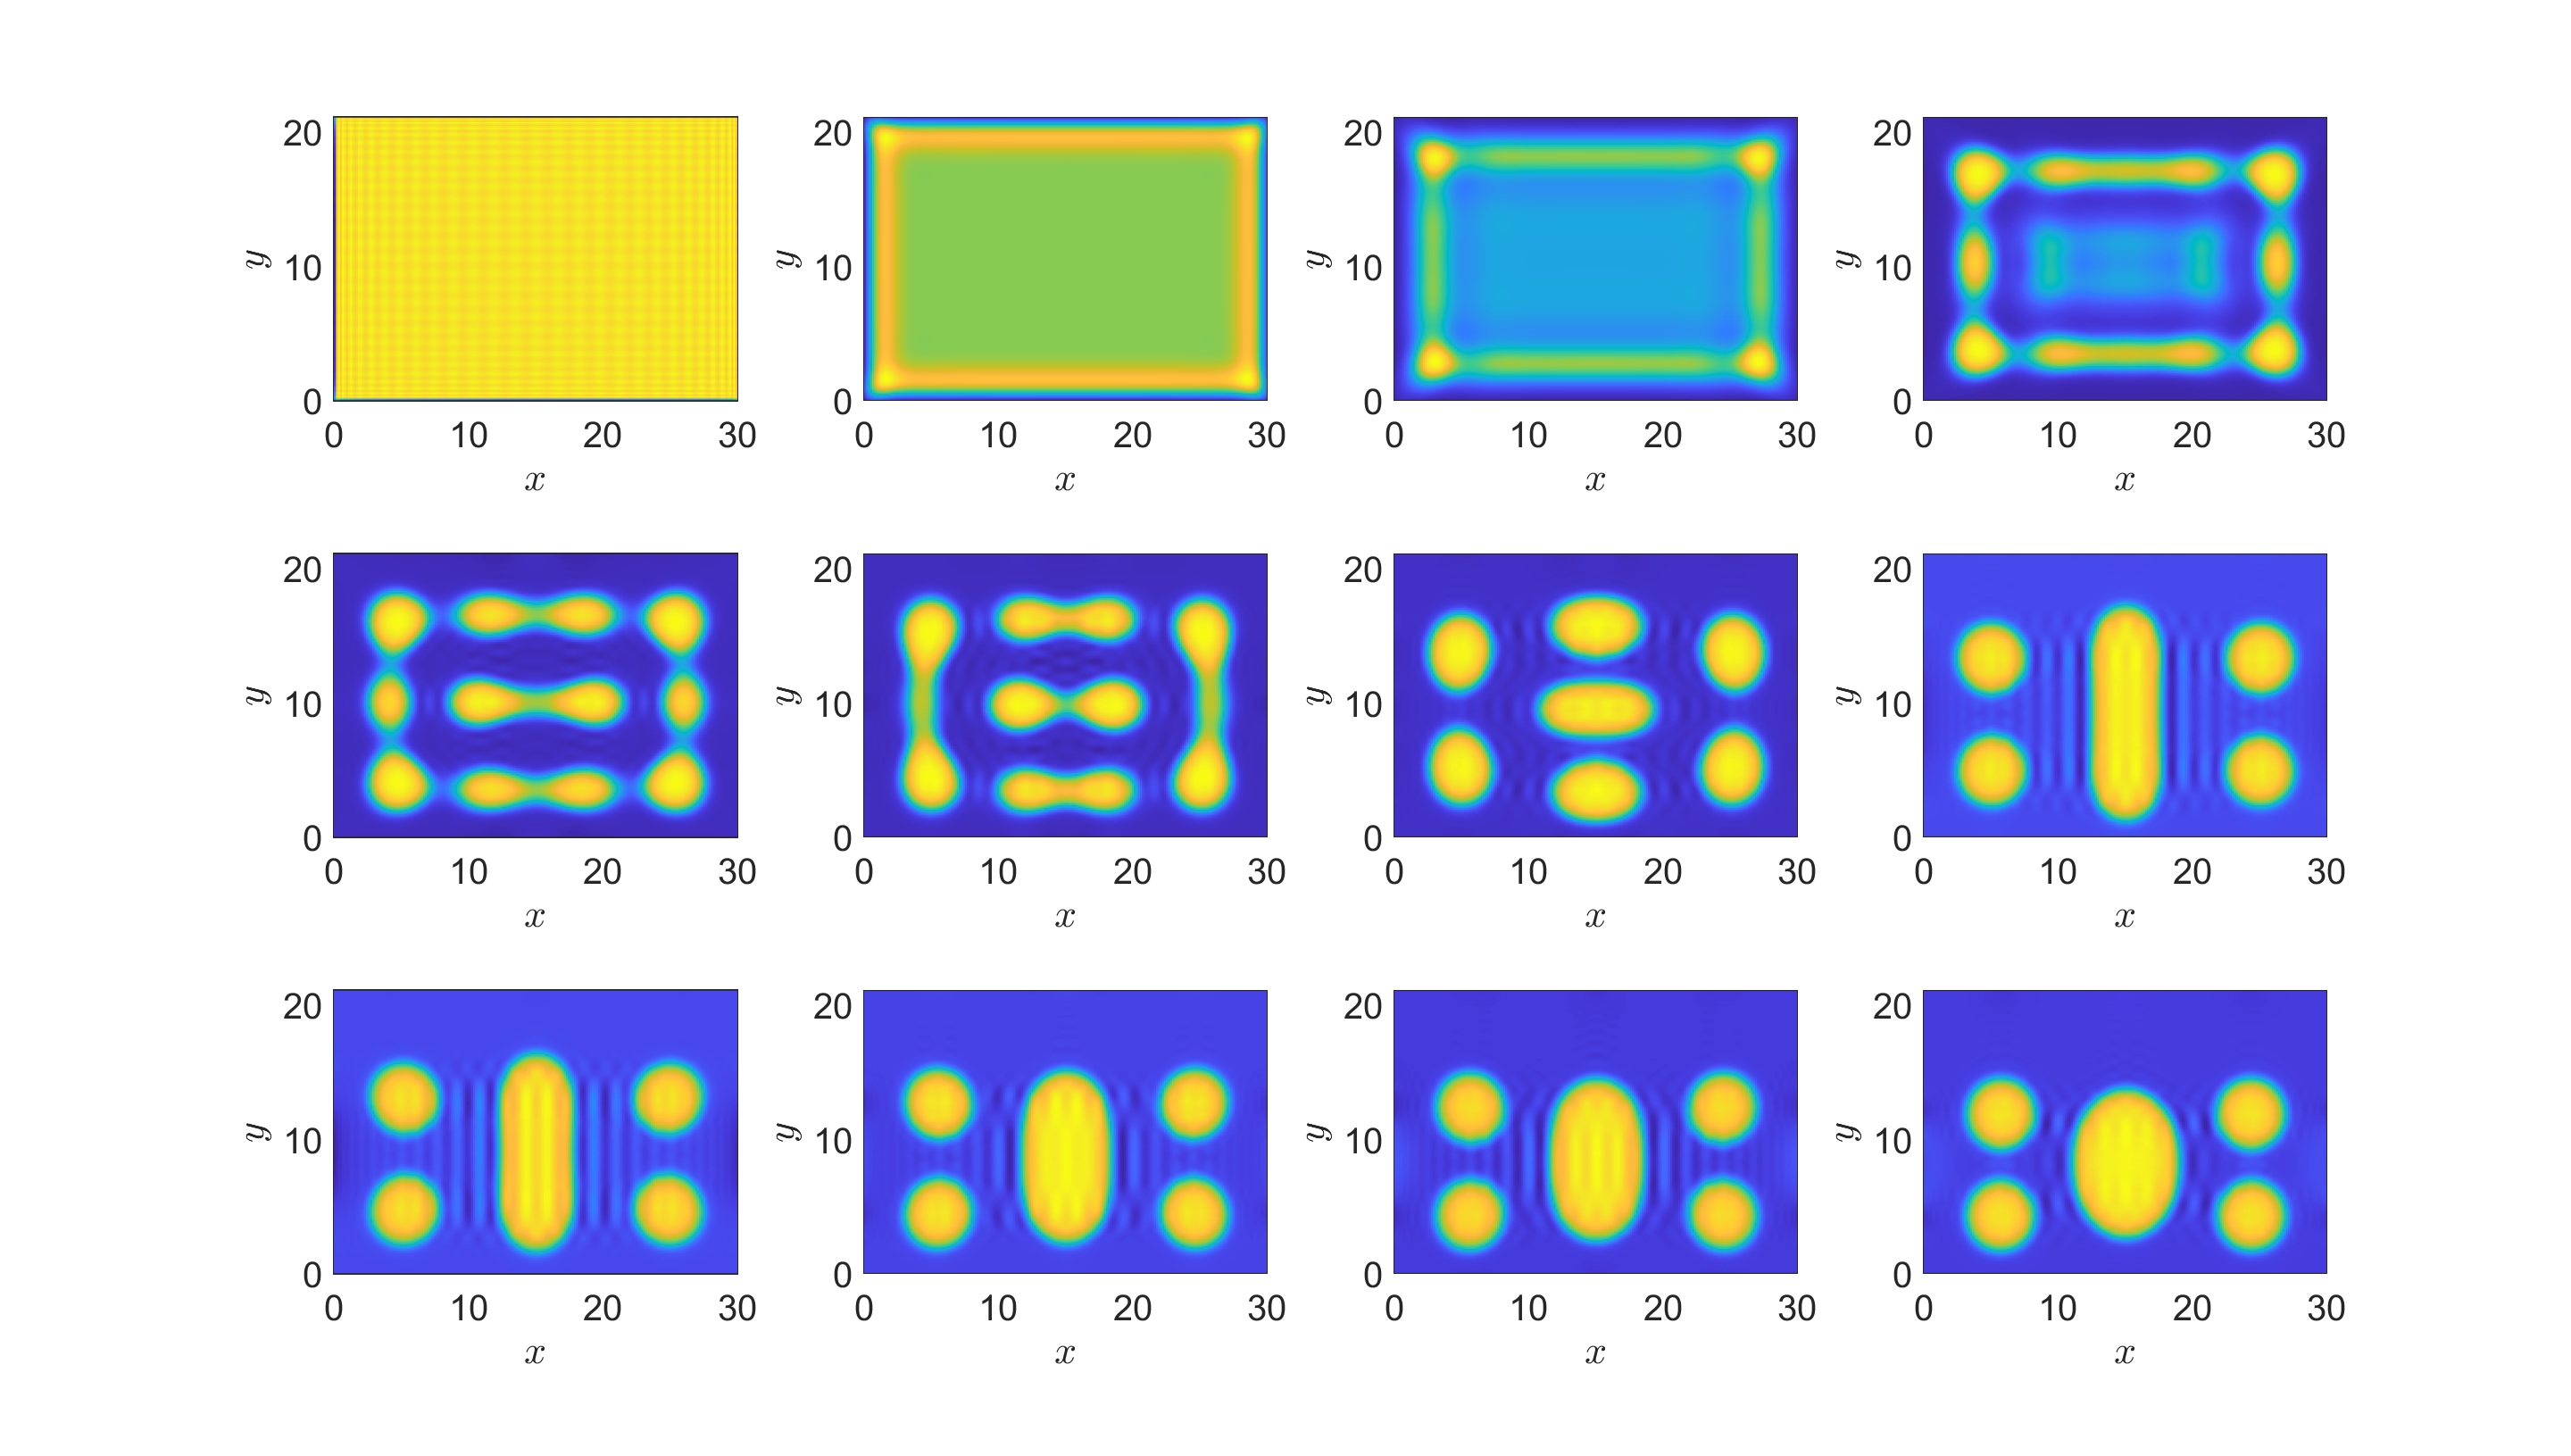
\includegraphics[scale=0.25]{Ex10F2.png}
		\caption{Figure 10 Example, $\bar \rho = 0.2$, $\sigma = 0.6$, $12$ different times} 
		\label{F4a}
	\end{figure} 
	
	
	
	\section{Flow Through Constrictions}	
	The setup is as in the paper by Zimmermann et al.
	The external potential is defined as:
	\begin{align*}
	V_{ext} &= V_0 [1 - 0.5erf((y+g(x))/\sqrt 2 w) + 0.5erf((y-g(x))/\sqrt 2 w)]\\
	g(x) &= L_y /2 - \alpha [1+ \cos(2\pi (x - x_0)/L_c)] \quad \text{for} \quad |x - x_0| < L_c/2,\\
	&= L_y /2 \quad \text{otherwise}\\
	 \alpha &= (L_y/4)(1-b),
	\end{align*}
	In the paper the constriction length is $2.686 l$, wall softness is $w = 0.25 l$ and $V_0 = 1000 k_BT$. The choice of channel height is $L_y = \sqrt \frac{\sqrt 3}{2} n l$, with $n = 5$ or $6$  and $L_x = 21.5 l$.  We choose $l = 1$.
	The average density is $\rho_0 = 1/l^2$. Their force is $f = k_bT/l$, which is constant one for us.
	They then run a forward problem without the force to equilibrate the system and use this as an initial condition for the forced version.
	I used the final time value of the unforced problem as the initial condition for the forced problem. Both forward problems took $30$ min to run with $n = 30$ and $N = 50$, which seems to be not quite enough, when inspecting the result, see Figure \ref{F5}. The modification here is that we take only a part of $L_x$, in particular $L_x = 6$ and therefore $\rho_0 = 1/36$. We choose $b = 0.9$. The external potential profile can also be seen in Figure \ref{F5}. One odd thing is that the barriers don't line up one to one.
	
	\begin{figure}[h]
		\centering
		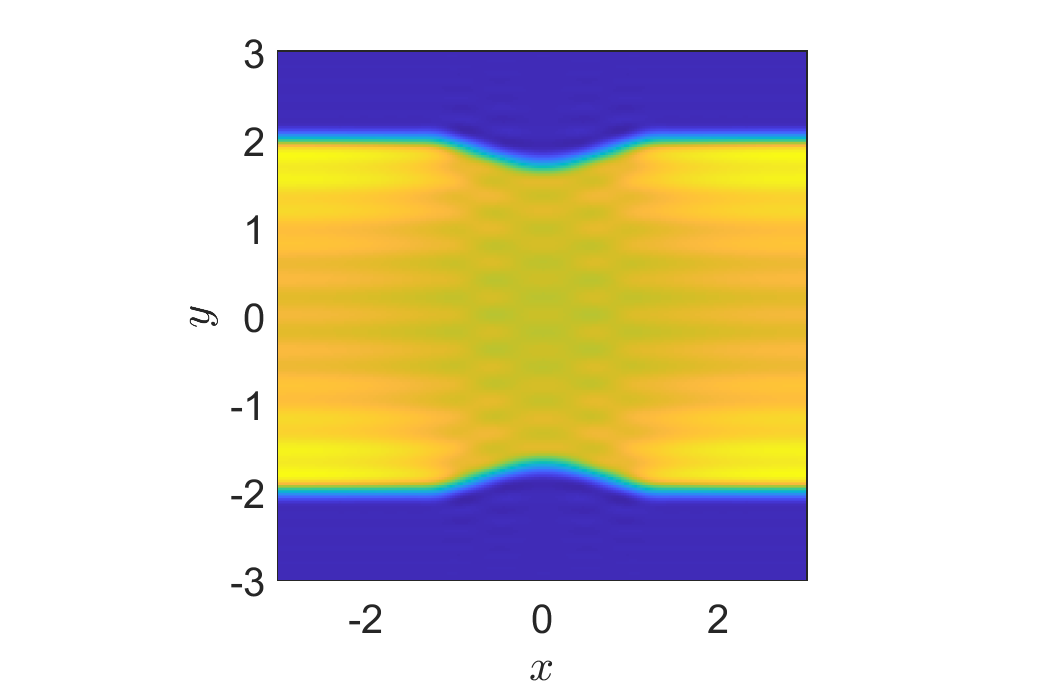
\includegraphics[scale=0.3]{Con1.png}
		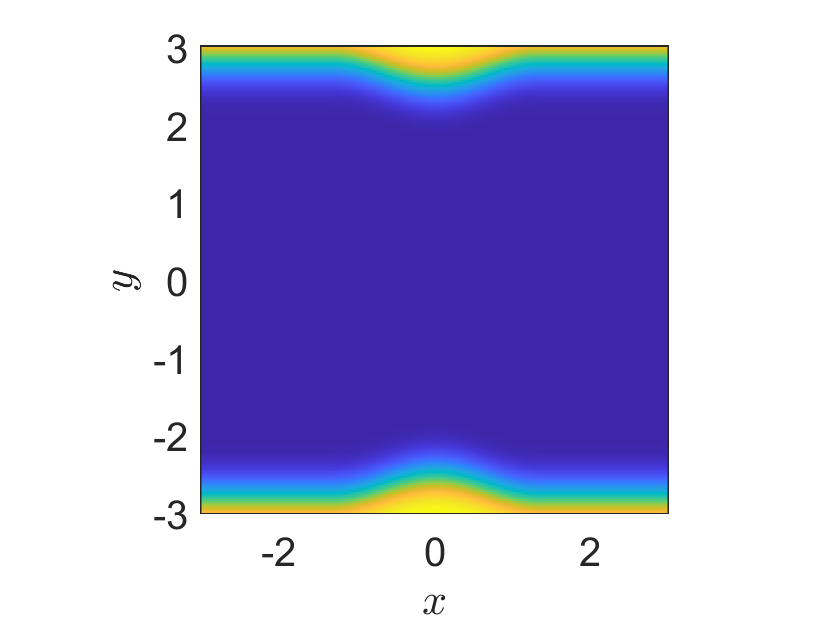
\includegraphics[scale=0.33]{Vext.png}
		\caption{Constriction Flow Equilibrium and corresponding $V_{ext}$} 
		\label{F5}
	\end{figure} 
	\begin{figure}[h]
		\centering
		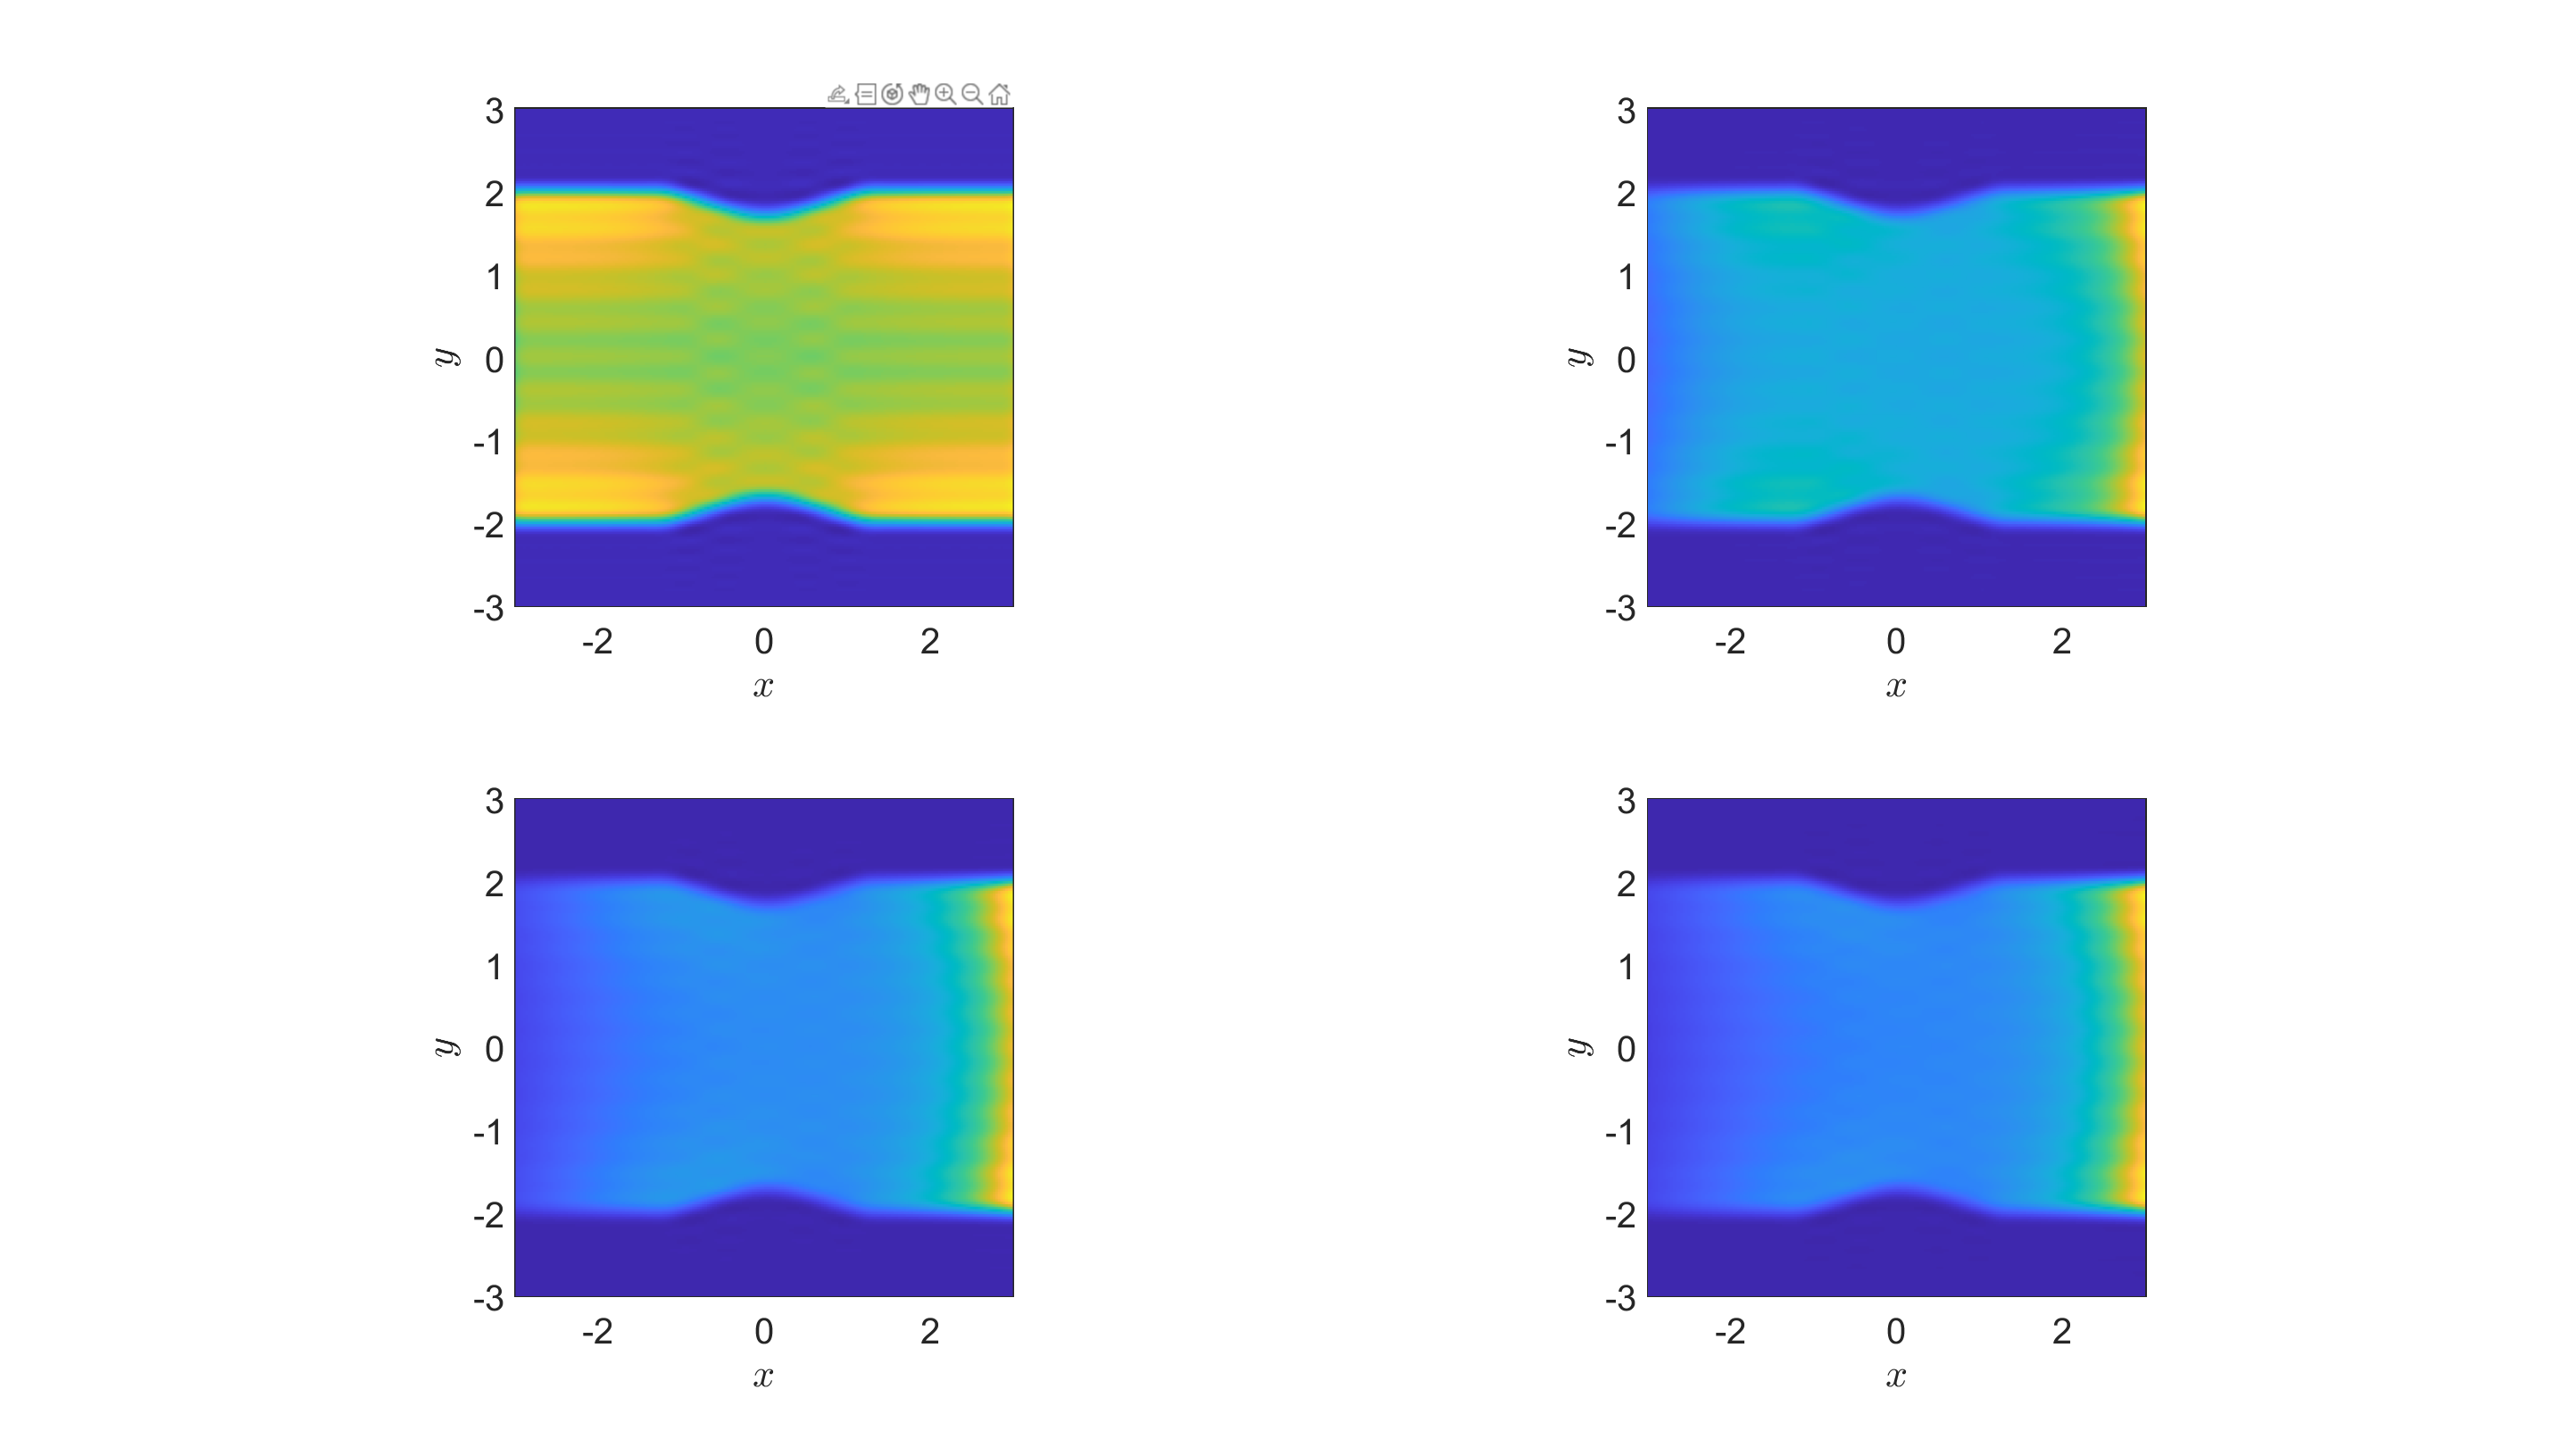
\includegraphics[scale=0.25]{Con2.png}
		\caption{Constriction Flow} 
		\label{F6}
	\end{figure} 

\end{document}